\documentclass{ltjbook}
\usepackage{docmute} 
\usepackage{../../myStyle} 

\begin{document}
\VerbatimFootnotes
\chapter{Descriptive Statistics}
\label{m05_descriptives}

So far, we have discussed why statistics is necessary in psychology, what computers are, and what kind of data is input into computers. That was the preparation. From here on out, we will delve into the specifics of psychological statistics.

First, allow me to introduce three frameworks in psychological statistics.
\begin{description}
    \item[記述統計 descriptive statistics] A statistical method for describing the characteristics of data, including visualization, summarization using representative values, etc. This is the first task to be done after collecting data, aiming to fully record what can be understood from the data at hand.
    \item[推測統計 inferential statistics] A branch of statistics that infers the overall picture from partial data. The purpose of psychological statistics is to predict the whole from a part of the sample. This will be the main topic in the second half (latter period) of this course.
    \item[多変量解析 multivariate analysis] A technique for extracting meaningful information from large amounts of data or eliminating meaningless information. This technique is used not only for survey research but also for handling data obtained from devices such as sensors. It is also an area that overlaps with data science, machine learning (so-called AI), etc. At this university, it will be covered in the second year's Applied Data Analysis course. 
\end{description}


As described here, descriptive statistics is the first step. The goal is to describe the characteristics of the data at hand. While visualizations can also be descriptive, this time we will focus on describing the characteristics of the data with numbers. Representative values for multiple data sets are referred to as representative values or measures of central tendency.

Let's say that you have quantified your research topic into numerical data. If your reaction was merely to admire the variety of digits, then that defeats the purpose of quantifying it. The basic step is to \textbf{present the data in a graph}. Make graphs right away, and make various kinds of them. As I mentioned last time, making graphs is a must. Now, it's important to analyze the data from the graphs. To summarize important features or differences in the data is even better. Therefore, you need to consider representative values.

It may seem blunt, but it is essentially impossible to represent a large set of data using just one representative value without modifying the TeX code. Because everyone is different, a dataset is significant precisely because of its diversity, and yet it is expressed as a single number. The representative value is determined by evaluating in some aspect, and it is nothing more than a representative value in that evaluation dimension. In other words, one representative value alone is not sufficient to understand the entire dataset. Also, making a single value representative means sacrificing some information. No matter what the representative value is, some information is always missing. Therefore, when dealing with statistical data, it is essential to use multiple representative values to make a multi-faceted judgement. Please keep this in mind and understand it well.

Without altering the TeX code, please allow me to translate the Japanese text into English:

"Then, these values can be classified into two types for explanation. One is an indicator of central tendency, and the other is an indicator of variability."

\section{Measures of Central Tendency}
\subsection{Mean}


You are a translator. 

"Mean, more precisely arithmetic mean, is probably the most well-known measure of central tendency. The calculation method involves adding all of the data together and dividing the sum by the number of data points."

Figure \ref{fig::04_01} shows the amount of money held by five individuals. In this example, the mean value can be calculated as follows.
\[ (15000+30000+20000+10000+20000)/5=19000 \]

\begin{figure}[ht]
    \centering
    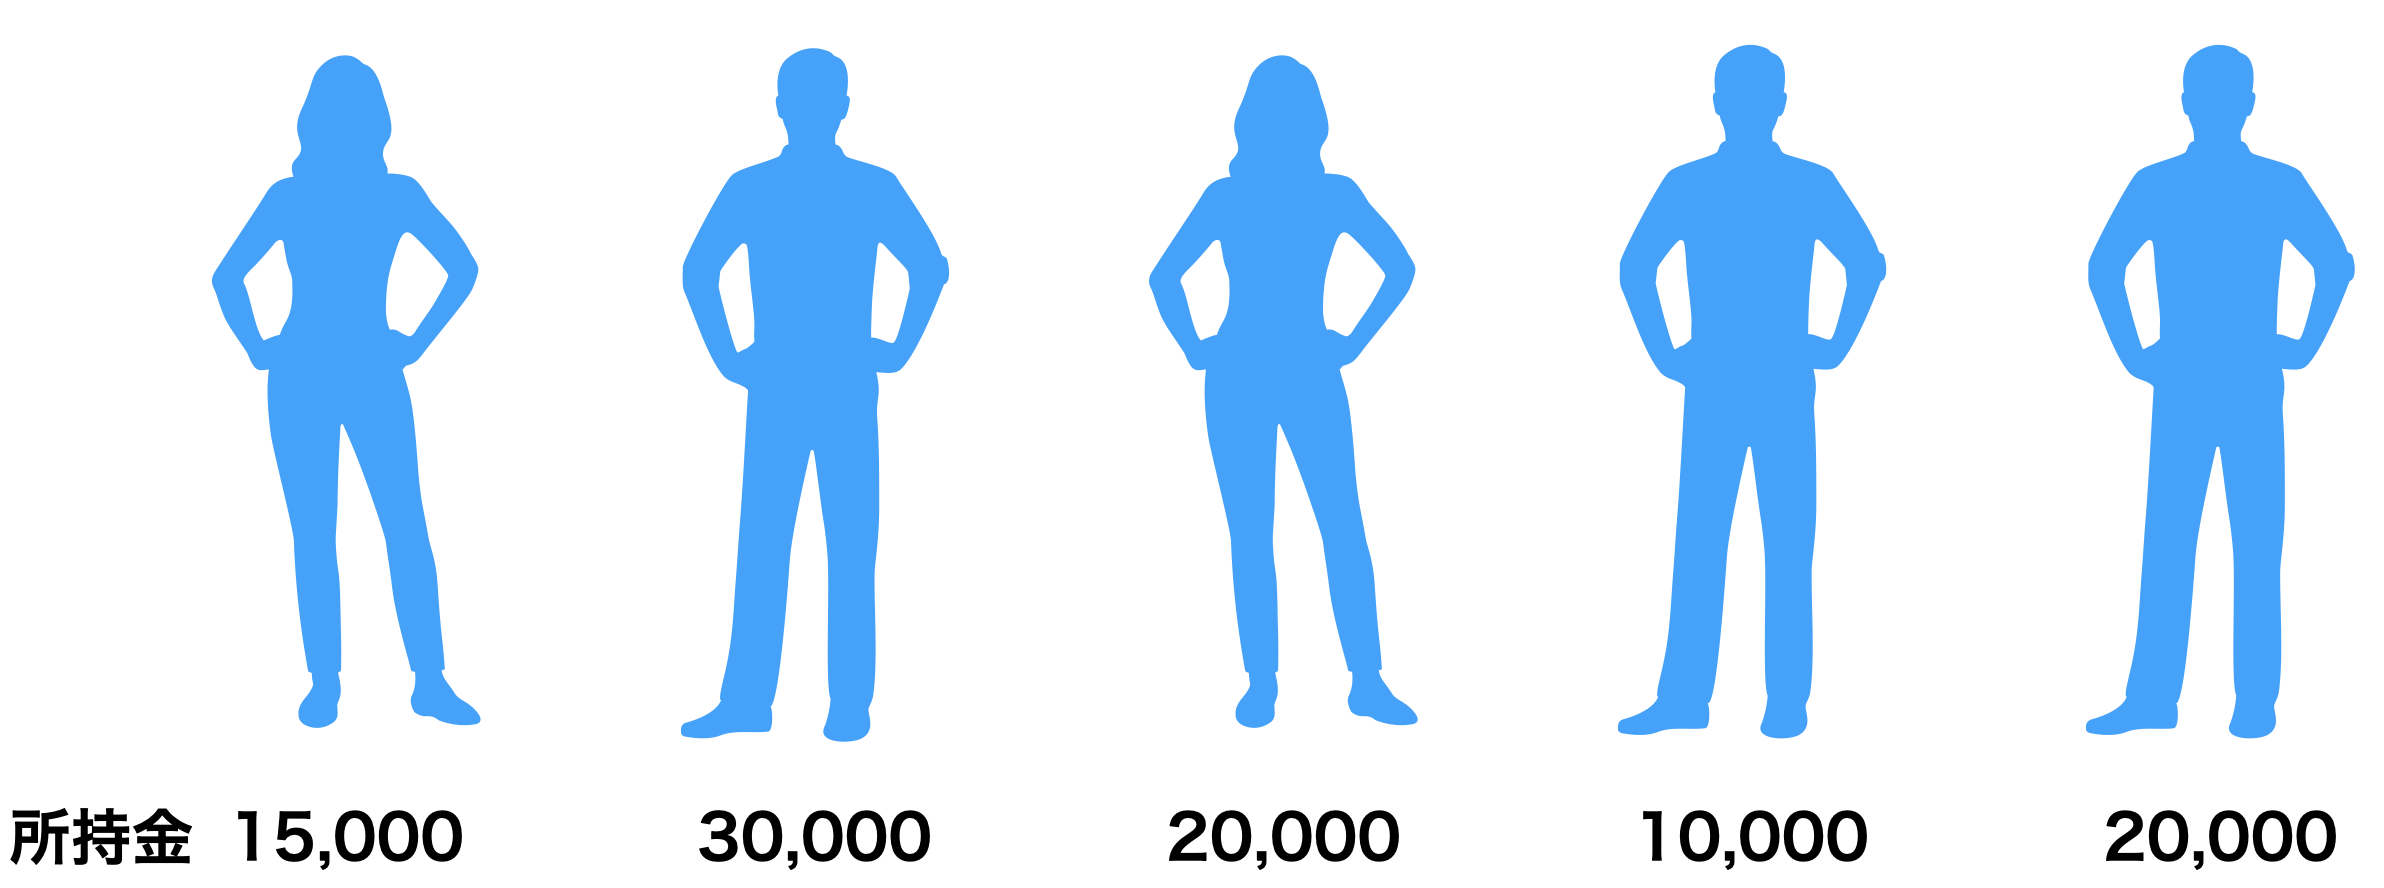
\includegraphics[keepaspectratio,width=0.8\linewidth]{../images/05_descriptives/slide04_01.png}
    \caption{Data on the amount of money possessed by 5 people}
    \label{fig::04_01}
\end{figure}


\paragraph{Introduction to characters and symbols}
Now let's learn the general notation for representing this using symbols in the future.
Variables are generally represented by $x$ or $y$ in mathematics.
There are data for five people in this case, and when referring to the differences between the data for the first person, the second person, and so on, we use subscripts indicated by small numbers placed slightly below and to the right of the alphabet, such as $x_1$, $x_2$, and so on. These are known as subscripts.
In this case, we had only one variable, which was the amount of money. However, in some cases, we may have many data and variables. In such cases, variables are represented by $x_{ij}$ with two subscripts. Here, $i$ represents the case (individual, observation number), and $j$ represents the variable number. \footnote{In this lecture, we follow this rule. There is not necessarily a rule that determines that the individual comes first and the variable comes later, but when introducing such symbols, it is common to specify which character corresponds to which. In this lecture, if it is not explicitly stated, please assume that the first subscript represents the individual and the second subscript represents the variable.}

I will now introduce the addition symbol. We will use $\sum$ to represent a summation. This symbol is the capital Greek letter S, and is derived from the first letter of the word "summation". It is read as "sum". We can add subscripts and superscripts to this symbol to give it meaning, as follows:
\[ \sum_{i=1}^5 x_i= x_1 + x_2 + x_3 + x_4 + x_5  \]
As shown here, there is a character "i" underneath the symbol $\sum$. This symbol represents the mathematical operation of adding up a sequence of values for the variable represented by "i" as it changes from 1 to 5. In the case of $\sum_{i=1}^5 x_i$, the variable $x_i$ changes as "i" ranges from 1 to 5, so the symbol implies adding up all the values of $x_i$ with changing subscripts. The symbol $\sum$ can also be used without explicitly stating the range of the variable when it is clear from context.

Now, let's talk about the average of the five numbers we mentioned earlier. The addition can be expressed as $x_1+x_2+\cdots+x_5=\sum_{i=1}^5 x_i$ without modifying the TeX code. Dividing this sum by 5 gives us the average, which is $\frac{1}{5}\sum x_i = 19000$. By using symbols like this, the average value can be generally expressed as follows.

\[ \bar{x} = \frac{1}{N}\sum_{i=1}^N x_i \]

We had five people this time, but it can be extended to handling $N$ data in general without modifying the TeX code. The left side is the average value $\bar{x}$, which is commonly denoted as x-bar.
\subsection{Median}


The following representative value is the \keytermE{median}: When data is sorted in order of size, the value of the middle case is used as the representative value. In the case of the previous figure \ref{fig::04_01}, when sorted, it becomes $10000<15000<20000=20000<30000$. The third item from the top (or bottom) is 20000 yen, so the median is 20000 yen.

This time, it happened to be a case of five people, so the middle was the third one, but there is a problem of what to do if there are only even numbers of data. In that case, it is common to use the arithmetic mean of the two values in the middle as the median.

\subsection{Mode, the most frequent value}
Finally, let's talk about the \keytermE{mode}{さいひんち}{最頻値} in statistics. As you can tell from the Kanji characters, the mode is the representative value that represents the most frequently occurring value among the data. In the case of the figure \ref{fig::04_01} presented earlier, only one person had 10000 yen, only one person had 15000 yen, and only one person had 30000 yen. However, since two people had 20000 yen, the mode becomes 20000 yen.

There are three different ways of thinking about the center of the data, and they do not necessarily agree with each other. Each one has its own significance, so it is necessary to consider them while comparing them.

Let's practice. If we have data like the one in Table \ref{tbl::04_01}, what would be the mean, median, and mode?

\begin{table}[ht]
    \centering
    \caption{Data for the amount of money held by 5 individuals (Part 2)}
    \begin{tabular}{lllll}
        A     & B     & C     & D     & E      \\\hline
        10000 & 10000 & 20000 & 25000 & 100000 \\
    \end{tabular}
    \label{tbl::04_01}
\end{table}


In this case, the mean is 33,000 yen, the median is 20,000 yen, and the mode is 10,000 yen. As you can see, the mean is higher than the other two values. This is because there is an outlier, E, who is significantly increasing the average. The mean takes into account the quantitative center point, so even if one person is far away from the rest, it can significantly affect the overall center. The median only considers the ordering information, so it simply recognizes the highest value regardless of the magnitude. The mode is based on frequency, so even if there is one wealthy person, it only counts as a frequency of 1. This reveals that the mean is weak against outliers, while the median and mode are robust against them.

Is the mean useless then? Of course not. If the data is symmetrically distributed, with values evenly spread out on both sides, then the mean is a good measure of central tendency. However, if the distribution of data is skewed, with values clustered on one side, the mean is not an appropriate measure of central tendency.

Figure \ref{fig::04_02} shows data obtained from the "National Living Basic Survey" conducted by the Ministry of Health, Labour and Welfare \footnote{\url{https://www.mhlw.go.jp/toukei/saikin/hw/k-tyosa/k-tyosa19/dl/03.pdf}}. Looking at this data, the income distribution is skewed to the left, with an average value of 5.523 million yen, but a median value of 4.37 million yen and a mode value in the 2-3 million yen class. The mode value represents the point with the most data, so when people are told that "the average national income is 5.52 million yen", many people (at least 55.9\% in this example) will feel the impression of "Is my annual income too low...?". Of course, the fact that the income distribution is skewed towards the lower end of the scale is also a bad situation, but it can be said that using the average value as a representative value is not appropriate in the first place\footnote{Of course, from the perspective of politicians, the fact that the average is 5.5 million yen means that Japan is wealthy, and it may be a good indicator to appeal to people with such numbers. There is no malice in the numbers, and the problem lies on the side of how people use what numbers in what way.}. In news coverage, only the average value is reported, but this can create an unfair impression. It is important to \textbf{visualize data} when discussing these issues.
\begin{figure}[ht]
    \centering
    
\includegraphics[keepaspectratio,width=0.8\linewidth]{../images/05_descriptives/slide04_02.png}
    \caption{Relative frequency distribution of households by income class}
    \label{fig::04_02}
\end{figure}


By the way, since the mode counts the frequency, when dealing with continuous numbers of an interval scale or higher, it is necessary to divide them into several intervals and count them. The example in Figure \ref{fig::04_02} is such a case. However, note that the mode's result can change depending on how the intervals are classified. The two histograms in Figure \ref{fig::04_03} actually represent the same data. The difference lies in how binwidth (the width of the intervals) is chosen: the left histogram has intervals of 15 points, while the right has intervals of 5 points. The modes are marked in red for each histogram, but in the left histogram, the mode is in the 40-55 point interval, whereas in the right histogram, it is in the 47-52 point interval. Therefore, you should also pay attention to the interval width when counting the mode.
\begin{figure}[ht]
    \centering
    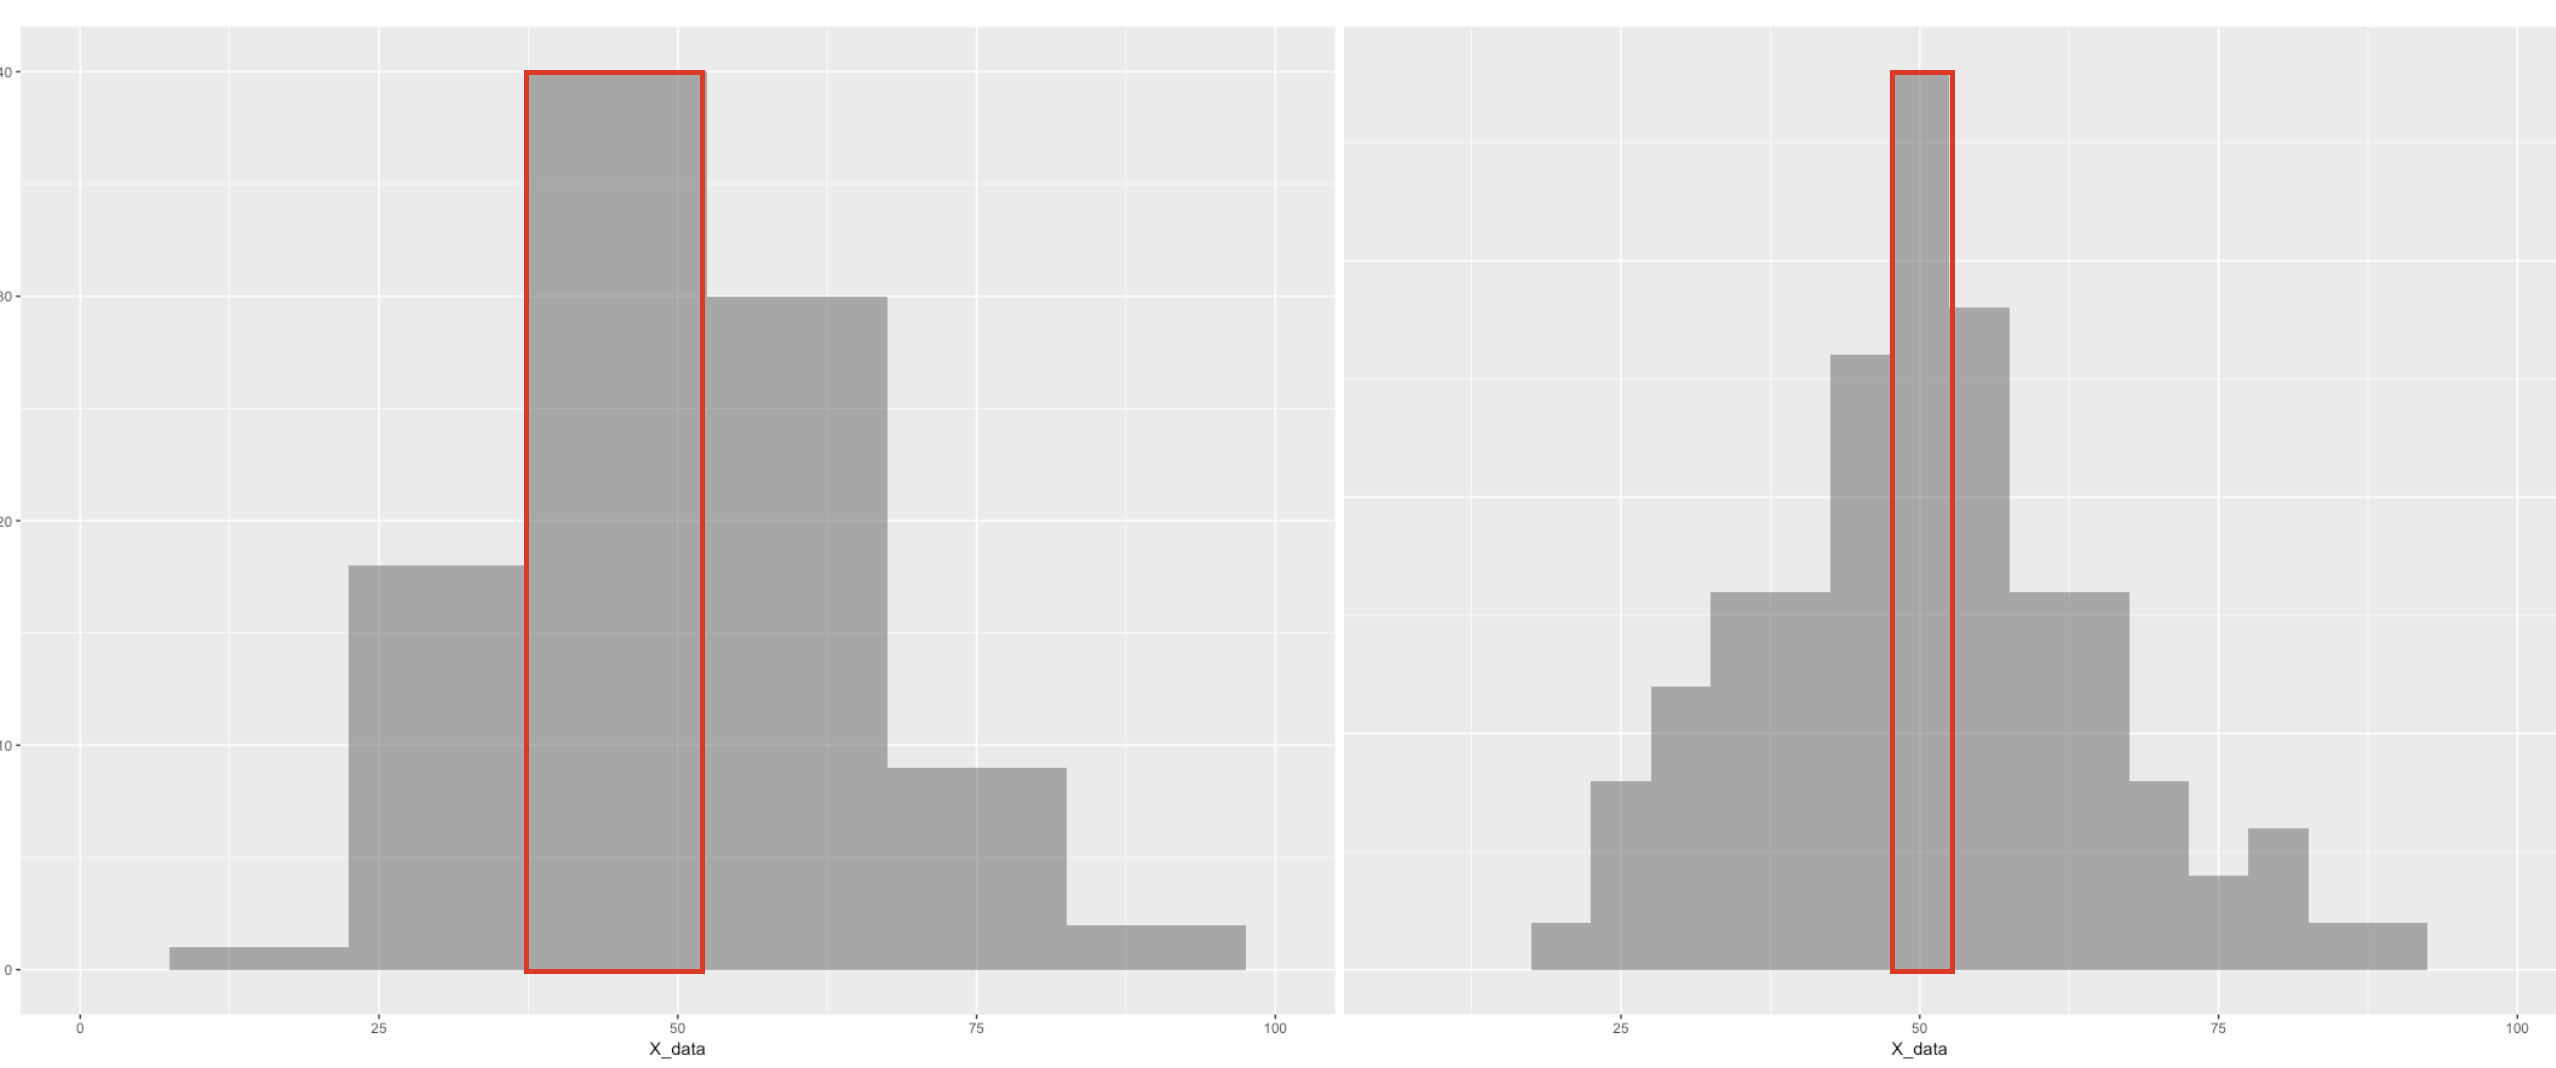
\includegraphics[keepaspectratio,width=0.8\linewidth]{../images/05_descriptives/slide04_03.png}
    \caption{The results change depending on how the interval width is divided.}
    \label{fig::04_03}
\end{figure}


Let's summarize the three indicators of centralization tendencies discussed here.

\begin{description}
	\item[平均値] The arithmetic mean uses all data and is a good indicator if there are no outliers; it is actually the most active indicator in statistical analysis. It is suitable for symmetric distributions.
	\item[中央値] The median is a less influenced indicator by outliers; it is easy to understand that it is exactly in the middle. However, only the middle number of the distribution is used. There are several ways to calculate the median when the data has an even number of items.
	\item[最頻値] The mode is less influenced by outliers and is easy to understand even when the distribution is not symmetrical. It only focuses on the frequency distribution, so it has the disadvantage that it changes when the interval width of the frequency distribution changes.
\end{description}


\section{Measures of Dispersion}
\subsection{Variance and Standard Deviation}
Next, let's consider the dispersion indicators. It is not always clear where the center of the data is just based on that information. Let's say we have two sets of data, like the ones shown in Table \ref{tbl::04_02}. This is illustrated in Figure \ref{fig::04_04}.

\begin{table}[ht]
    \centering
    \caption{Two Data Sets}
    \begin{tabular}{ll}
        A & B \\\hline
        4 & 1 \\
        4 & 2 \\
        5 & 3 \\
        5 & 5 \\
        5 & 5 \\
        5 & 7 \\
        6 & 8 \\
        6 & 9 \\\hline
    \end{tabular}
    \label{tbl::04_02}
\end{table}


\begin{figure}[ht]
	\centering
	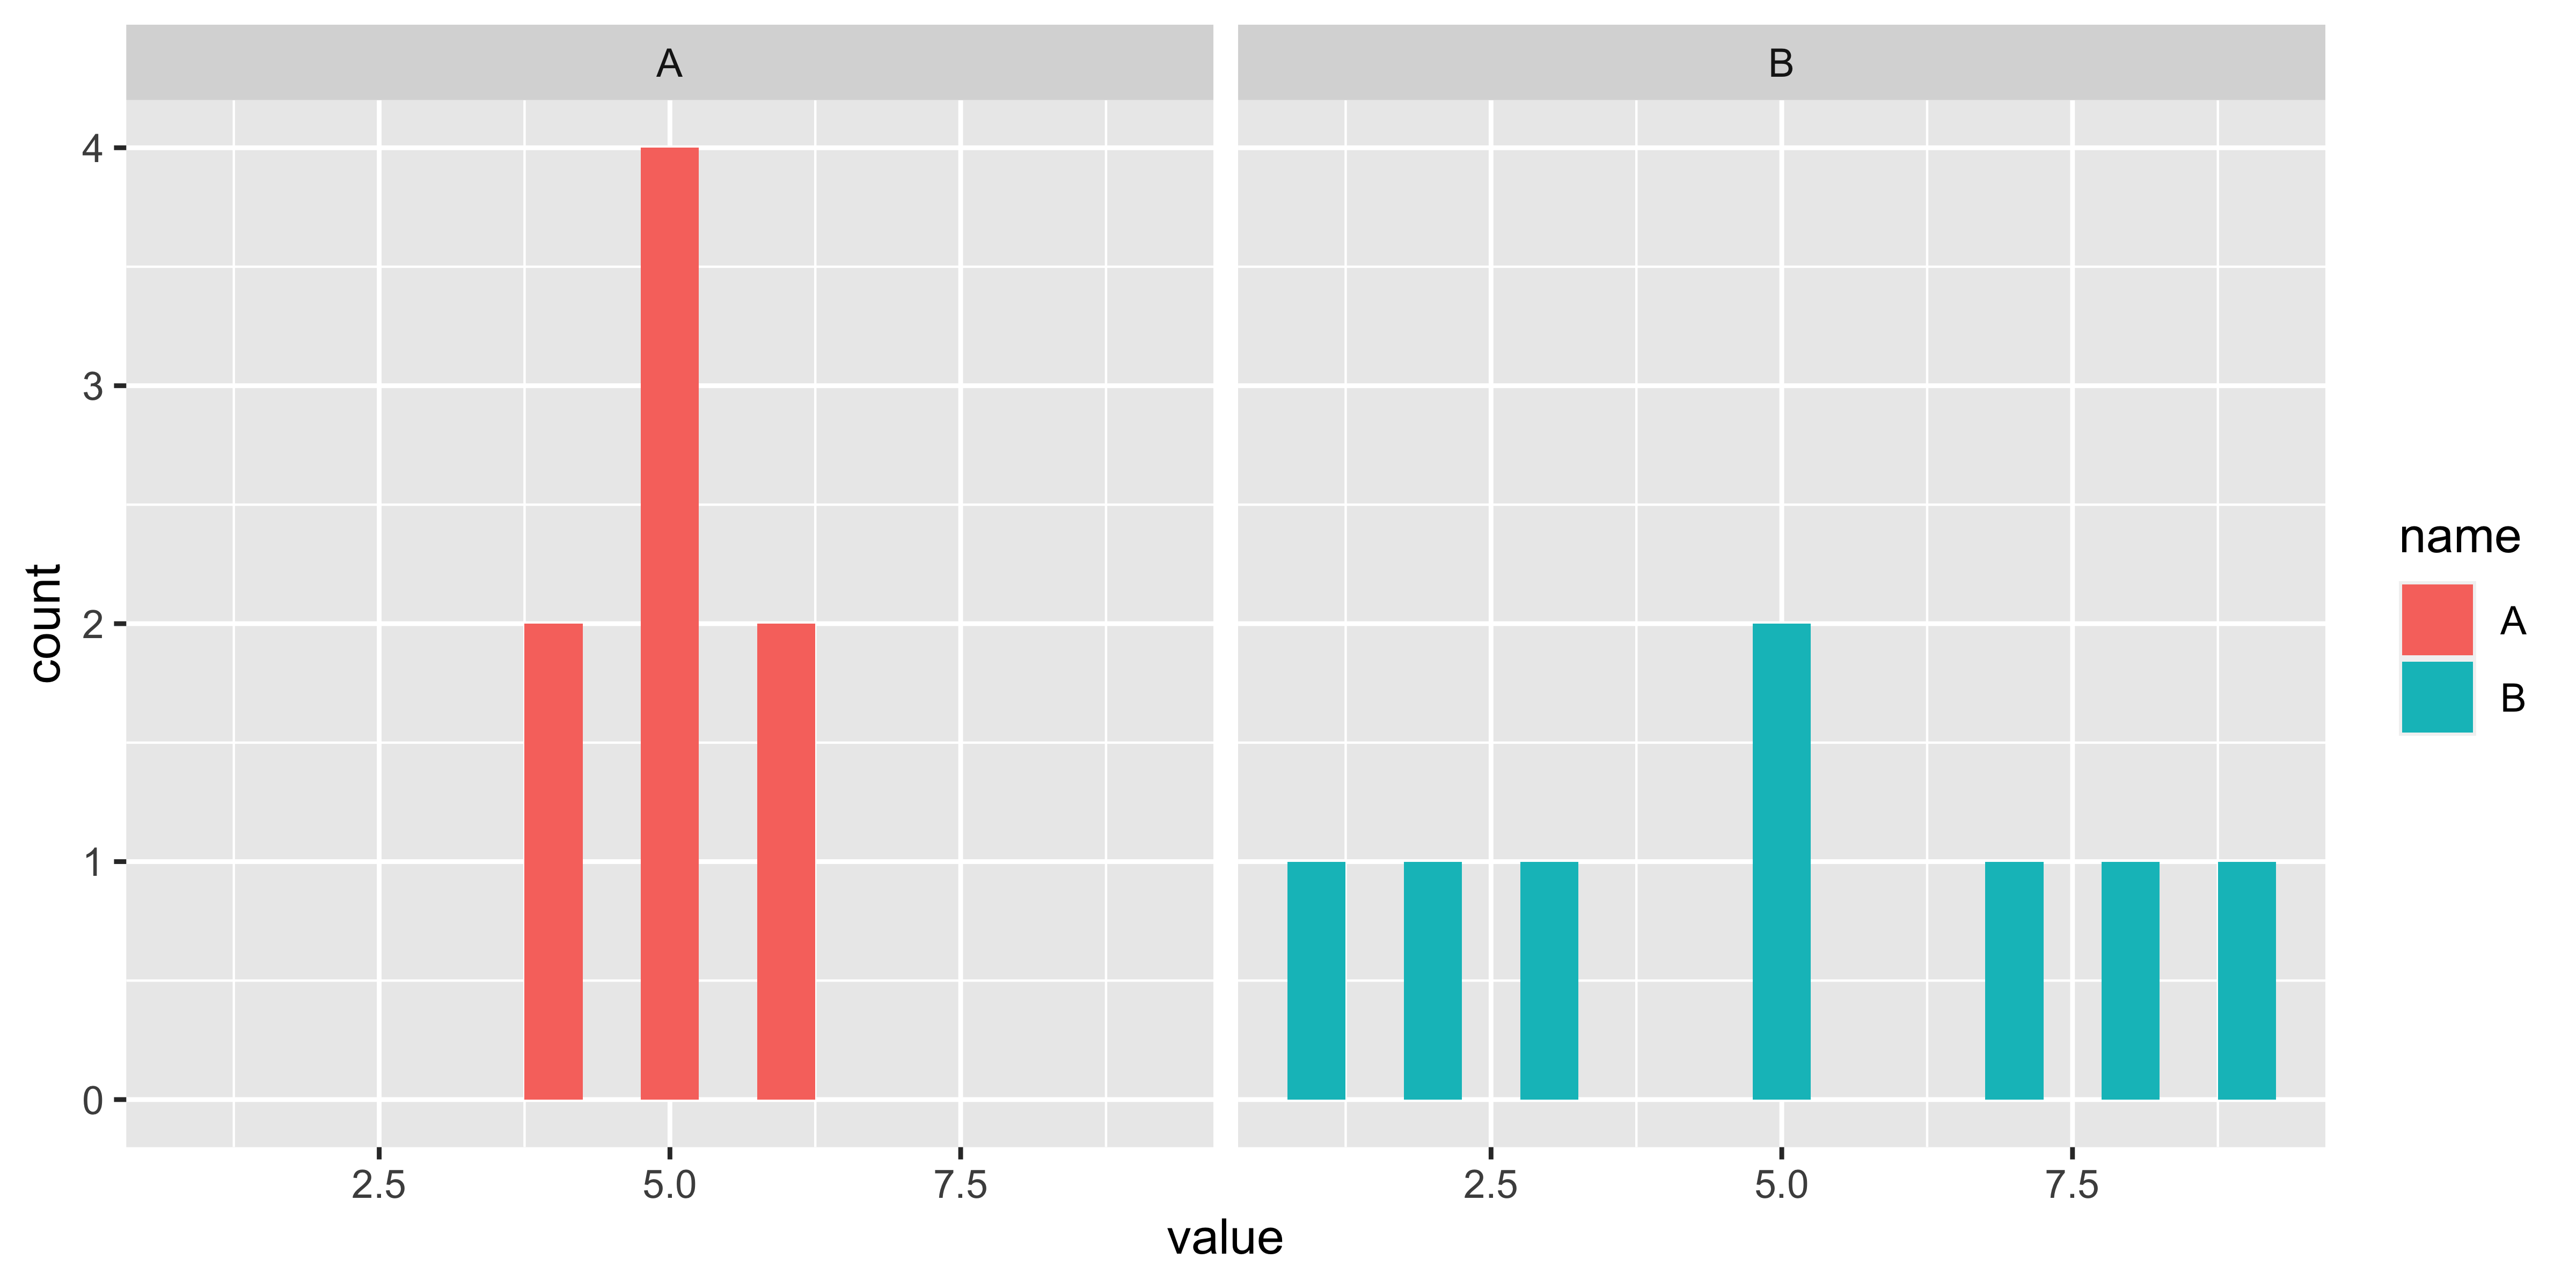
\includegraphics[keepaspectratio,width=0.8\linewidth]{../images/05_descriptives/Rplot04_01.png}
	\caption{Let's compare two data sets.}
	\label{fig::04_04}
\end{figure}


What would happen to the averages, medians, and modes of groups A and B for this data? Surprisingly, both groups have an average of 5, a median of 5, and a mode of 5. Using measures of central tendency alone does not express the difference between Group A and Group B. Even though they have such different appearances!

As for the difference between these two groups, as is evident from Figure \ref{fig::04_05}, the degree of scattering from the center to the left and right is different.

\begin{figure}[ht]
    \centering
    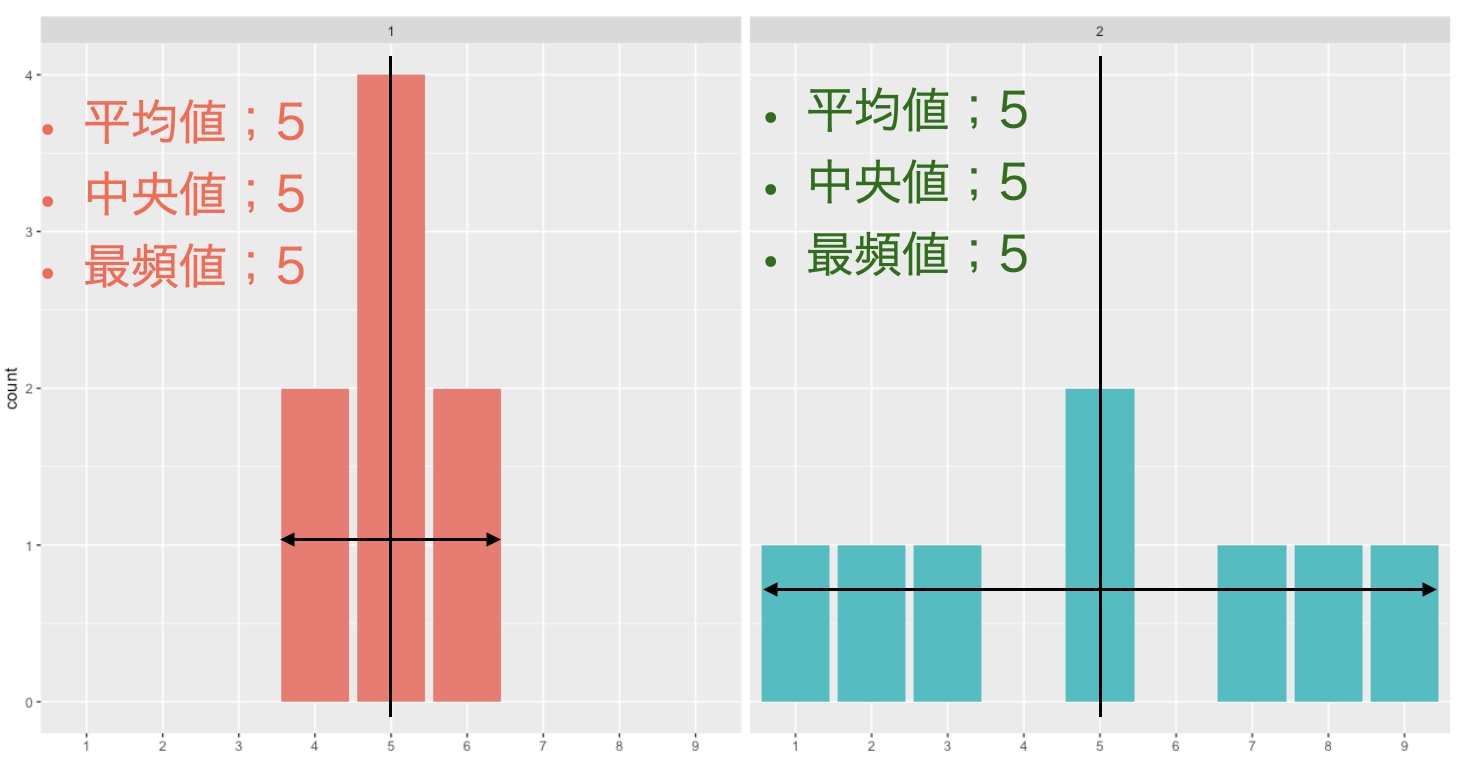
\includegraphics[keepaspectratio,width=0.8\linewidth]{../images/05_descriptives/slide04_05.png}
    \caption{How far each data point is on average from the center}
    \label{fig::04_05}
\end{figure}


"Distribution"
The representative value that expresses this well is the variance, which is the "degree to which individual data points are typically separated from the mean." The key point of quantification is to consider how far each individual data point is from the center. This is expressed mathematically as follows:

\[ s_x^2  = \frac{1}{N}\sum_{i=1}^N (x_i - \bar{x})^2 \]

The term $(x_i - \bar{x})$ in this equation represents how far each data point $x_i$ is from the mean $\bar{x}$. This is called the \textit{mean deviation}. The term is then squared. The reason for this is important: if we do not square the value, then the sum of the mean deviations would always be zero\footnote{Try it out!}. This is because the positive and negative values would cancel each other out. Squaring the value removes the sign, so that we do not lose any information\footnote{We could also use the absolute value, but it is hard to express this symbolically in equations.}

Shall we actually calculate it? The variance of group A is as follows:
\[ \frac{1}{8}((4-5)^2+(4-5)^2+(5-5)^2+(5-5)^2+(5-5)^2+(5-5)^2+(6-5)^2+(6-5)^2) \]
\[ =\frac{1}{8}(1^2+1^2+0^2+0^2+0^2+0^2+1^2+1^2) = \frac{4}{8}=0.5\]
The variance of group B is as follows.
\[ \frac{1}{8}((1-5)^2+(2-5)^2+(3-5)^2+(5-5)^2+(5-5)^2+(7-5)^2+(8-5)^2+(9-5)^2)\]
\[ =\frac{1}{8}(4^2+3^2+2^2+0^2+0^2+2^2+3^2+4^2) = \frac{58}{8}=7.25 \]
As we can see, the variance of Group A is 0.5, while that of Group B is 7.25, indicating that Group B has a larger dispersion.

Variance represents the dispersion of data. The larger the variance, the greater the dispersion of the data.
On the other hand, when the variance becomes zero, it means that there is no dispersion in the data.
If the variance of the actual data is zero, it means there is no information to be obtained from it.
Because, for example, if all students in a class score 100 on a test, the variance is 0. In this case, we cannot gain insights such as "what kind of studying leads to better grades?" or "how can we support students with lower grades?" from it. In a dataset with a variance of 0, there are no individual differences, so we cannot obtain any useful information. In other words, variance is a crucial indicator in that it represents the maximum amount of "meaning" or "information" that can be obtained from the data!

By the way, the equation for dispersion can be expanded as follows:
\[
Please translate this Japanese text into English without changing the TeX code:
You are a translator. 

Please translate this Japanese text into English without modifying the TeX code:

        s_x^2 & = & \frac{1}{N}\sum_{i=1}^N (x_i - \bar{x})^2
You are a translator.
You are a translator. 

Please translate this Japanese text into English without modifying the TeX code:

              & = & \frac{1}{N}\sum_{i=1}^N (x_i^2 - 2x_i\bar{x} + \bar{x}^2)                                                                           \\
&   &                                                                                                          & \mbox{The summation symbol can be distributed, so}\\
& = & \frac{1}{N}\sum_{i=1}^N x_i^2 - 2\frac{1}{N}\sum_{i=1}^N x_i\bar{x} + \frac{1}{N}\sum_{i=1}^N \bar{x}^2) \\
&=& \frac{1}{N} \sum_{i=1}^N x_i^2 - \frac{2}{N} \bar{x} \sum_{i=1}^N x_i + \frac{1}{N} \bar{x}^2 \sum_{i=1}^N 1 \\
&=& \frac{1}{N} \sum_{i=1}^N x_i^2 - 2\bar{x}^2 + \bar{x}^2 \\
&=& \frac{1}{N} \sum_{i=1}^N x_i^2 - \bar{x}^2 \\
where && \bar{x} = \frac{1}{N} \sum_{i=1}^N x_i
& & & \mbox{Adding a constant N times is equivalent to multiplying by N.}
You are a translator. 

Please translate this Japanese text to English without modifying the TeX code: 

              & = & \frac{1}{N}\sum_{i=1}^N x_i^2 - 2\frac{1}{N}N\bar{x}\sum_{i=1}^N x_i + \frac{1}{N}N\bar{x}^2)
Please translate this Japanese text into English without modifying the TeX code: 

              &   &                                                                                                                                                     \\
You are a translator. 

Translate this Japanese text into English without modifying the TeX code:

              & = & \frac{1}{N}\sum_{i=1}^N x_i^2 - 2\bar{x}\frac{1}{N}\sum_{i=1}^N x_i + \bar{x}^2)
Please translate this Japanese text into English without modifying the TeX code:
You are a translator.

& = & \frac{1}{N}\sum_{i=1}^N x_i^2 - 2\bar{x}\bar{x}+ \bar{x}^2)
Please translate this Japanese text into English without modifying the TeX code: 

               &   &                                                                                                                                     \\
You are a translator.

(Note: This sentence does not include any TeX code and therefore cannot be translated using TeX commands.)
Please translate this Japanese text into English without modifying the TeX code: 

             &   &                                                                                                                                                     \\
You are a translator. 

& = & \frac{1}{N}\sum_{i=1}^N x_i^2 - \bar{x}^2
You are a translator.
\]
When performing calculations, it may be faster to first square all variables and compute the average, so this is often done. However, in today's world with the advancement of electronic computers, the need for manual calculation of variance has diminished significantly.
Standard Deviation
By the way, the variance is calculated from the squared values of the original data. Therefore, it is important to note that the units of variance are different from the original scale. That is, if the original data was in units of cm, then the variance is in units of $cm^2$. As a result, the numbers tend to get larger and it can be difficult to grasp the magnitude of the variance. This is a disadvantage of using the variance as a measure of dispersion.

So let's consider converting the units back to their original form. Since they have become larger by being squared, taking the square root should bring them back to their original values.
\[ s_x = \sqrt{\frac{1}{N}\sum_{i=1}^N (x_i - \bar{x})^2} \]
The computed $s_x$ as shown is known as the \keytermE{standard deviation}, and is abbreviated as SD. Since taking the square root is all that is required, this can be computed rapidly. For example, in the previous case, the SD for group A is 0.7071, and for group B is 2.6925.


\paragraph{Quartiles and IQR}
There are other indicators to express the range. While the variance and standard deviation are indicators related to the mean value, there is an indicator called "quantile" that is related to the median. Literally, it refers to the number that corresponds to the dividing point when the data is divided into four parts.
The median is defined as the middle number when the data is arranged in ascending order, but when the data is divided into quarters, as shown in Figure \ref{fig::04_06}, the lower quarter is called the first quartile and the upper quarter is called the third quartile. This means that the median is the same as the second quartile.

\begin{figure}[ht]
	\centering
	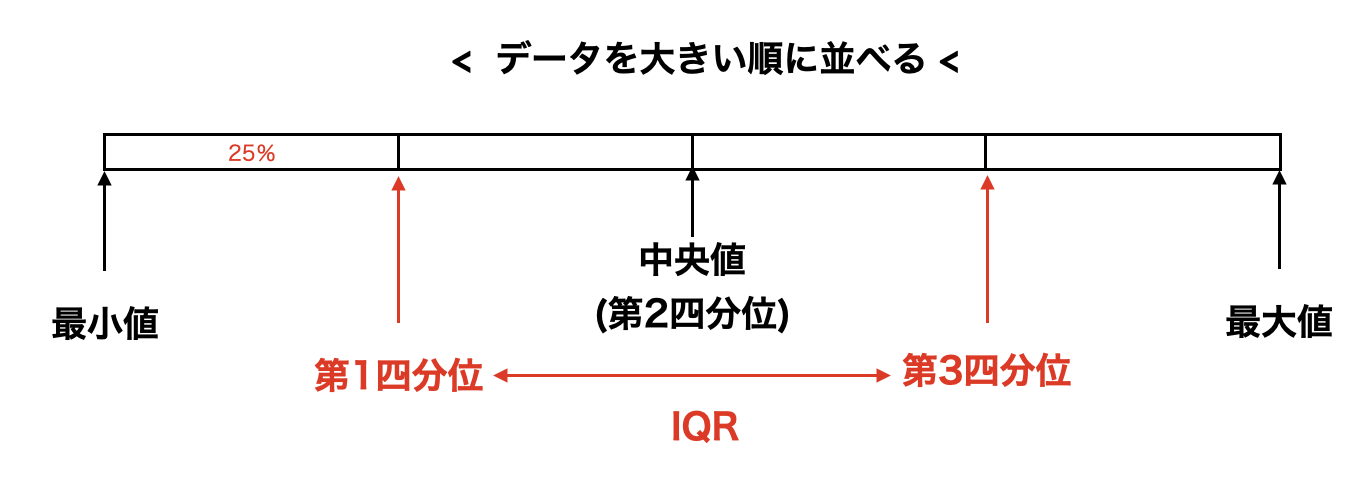
\includegraphics[keepaspectratio,width=0.8\linewidth]{../images/05_descriptives/slide04_06.png}
	\caption{Quartiles and IQR}
	\label{fig::04_06}
\end{figure}


The width using the first quartile and the third quartile, that is, the number obtained by subtracting the first quartile from the third quartile, is called the Interquartile Range (IQR). It is a simpler measure than the mean which is less affected by outliers and easy to understand since it is in the same units as the original data, unlike the standard deviation.
Now, some people may prefer not a four-part division but a five-part division. Or maybe even a three-part division would be fine. The point is, it's possible to consider values divided in some ratio. This is referred to as the "percentile," which represents a value corresponding to some ratio. For example, the first quartile is the same as the 25th percentile and the third quartile is the same as the 75th percentile. If this expression can be used, it is possible to divide it by any number. Depending on the shape of the distribution, it may also be necessary to display values such as the 95th percentile or the 5th percentile.

In Chapter \ref{m04_usingR}, we mentioned box plots. You may have learned about them under the name "box-and-whisker plots" in high school mathematics. This method of visualization represents the range of data using boxes and whiskers. Typically, the middle line of the box represents the median, the lower line represents the first quartile, and the upper line represents the third quartile. However, there are two ways to represent the whiskers. Figure \ref{fig::04_07} shows the same data with two different methods: one is to represent the whiskers as the "maximum and minimum values" (top), and the other is to represent them as "up to 1.5 times the interquartile range (IQR)" (bottom). Please note which method is being used, as in the context of data analysis, the latter method is more commonly used to represent outliers with a dot beyond the whiskers. While there is no definitive "right" way between these methods, we remind you of the latter method as it is more frequently used in the future.
\begin{figure}[ht]
    \centering
    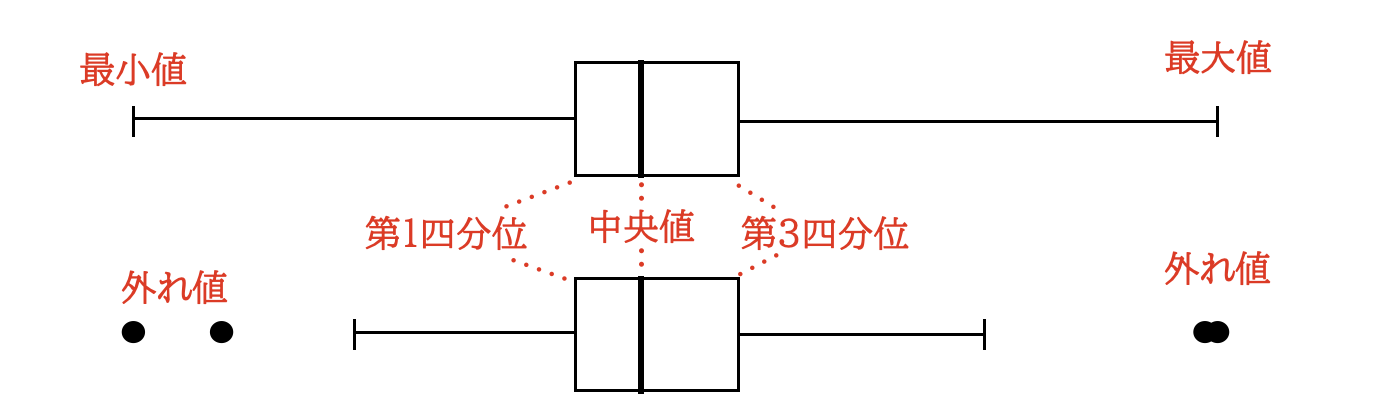
\includegraphics[keepaspectratio,width=0.8\linewidth]{../images/05_descriptives/slide04_07.png}
    \caption{Two types of box plots}
    \label{fig::04_07}
\end{figure}

\paragraph{Maximum, Minimum, Range}
Here we introduce the simplest measures of dispersion for numerical data. The \keytermE{maximum}{さいだいち}{Max} refers to the largest value in the data, whereas the \keytermE{minimum}{さいしょうち}{Min} is the smallest value. The \keytermE{range}{はんい}{Range} is simply the difference between the maximum and minimum values. Easy enough, right?


So far, we have explained the indicators of central tendency and scatter. As mentioned earlier, these representative values have limitations in expressing the data. In papers and other documents, it is essential to first provide descriptive statistics for the acquired data. By describing the mean, median, standard deviation, maximum and minimum values of the data, you can understand what kind of data it was (without having to write down all the data points). On the other hand, using only the mean value alone is insufficient as it only represents the middle of the data, and it's impossible to determine if the data is skewed. Additionally, if the data is not symmetrical, statistical analysis techniques frequently used may not apply. Ignoring this fact and analyzing the data carelessly may lead to incorrect conclusions. Please do not hesitate to view the data from different angles (display and confirm multiple representative values). Fortunately, many statistical packages can instantly calculate these values, so there is no need to struggle with the calculation.

\section{Relative Positions of Data}
\label{zScore}
Now we can view the entire dataset through representative values. We can now see the mean and standard deviation here, but let's consider using them to represent the relative position of each data point.

Many of the objects of study in psychology do not have an absolute zero point. For example, when considering personality, there is no such thing as a personality trait that simply "does not exist." Of course, there are people who are brighter, more diligent, or more emotionally unstable than others. However, these are all relative positions among many people, and there is no person who does not exist on a dimension of brightness or darkness simply because they are not bright. In other words, at best, the data features an interval scale level. When considering these traits in comparison to others, it is necessary to think about ways to express relative positions.

Let's assume that we place the center point that determines the relative position at the average value, since there is no zero point. "The deviation from the average" can be expressed as $x_i - \bar{x}$, so the data on a student's grades is presented in Table \ref{tbl::04_03}.  Looking at this, you might think that this person is good at English because their score is the highest. However, when compared to the class average, it's actually lower, surprisingly revealing that they may not be good at English relatively. It's difficult to rely solely on the raw scores\footnote{At the junior high school my daughter attended, they showed us a printout summarizing her test results, but it only displayed her raw score and average score, making it a completely meaningless list of numbers. I told her to protest to the school, but it was never fixed until she graduated.}. Now, looking at the deviation, we see that the average deviation for both Japanese and math is +14. Although we may want to consider that Japanese and math are equally good, is this way of thinking really valid?
\begin{table}[ht]
	\centering
	\caption{Comparison of Grades}
	\begin{tabular}{ccccc}
		Subject     & Grade $X_i$ & Class average $\bar{X}$ & Deviation ($x_i - \bar{x}$) & Standard deviation ($s_x$) \\\hline
		English     & 86          & 90                      & -4                          & 8                          \\
		Japanese    & 67          & 53                      & 14                          & 10                         \\
		Mathematics & 44          & 30                      & 14                          & 5                          \\
	\end{tabular}
	\label{tbl::04_03}
\end{table}

Actually, this is still not enough. This is because when we look at the standard deviation of this class, there is about a twofold difference between Japanese and math. The difference in standard deviation is due to the difference in the distribution of the data. We have plotted this in Figure 4.8. This is an example of the scores of this test assuming a symmetric distribution.

\begin{figure}[ht]
	\centering
	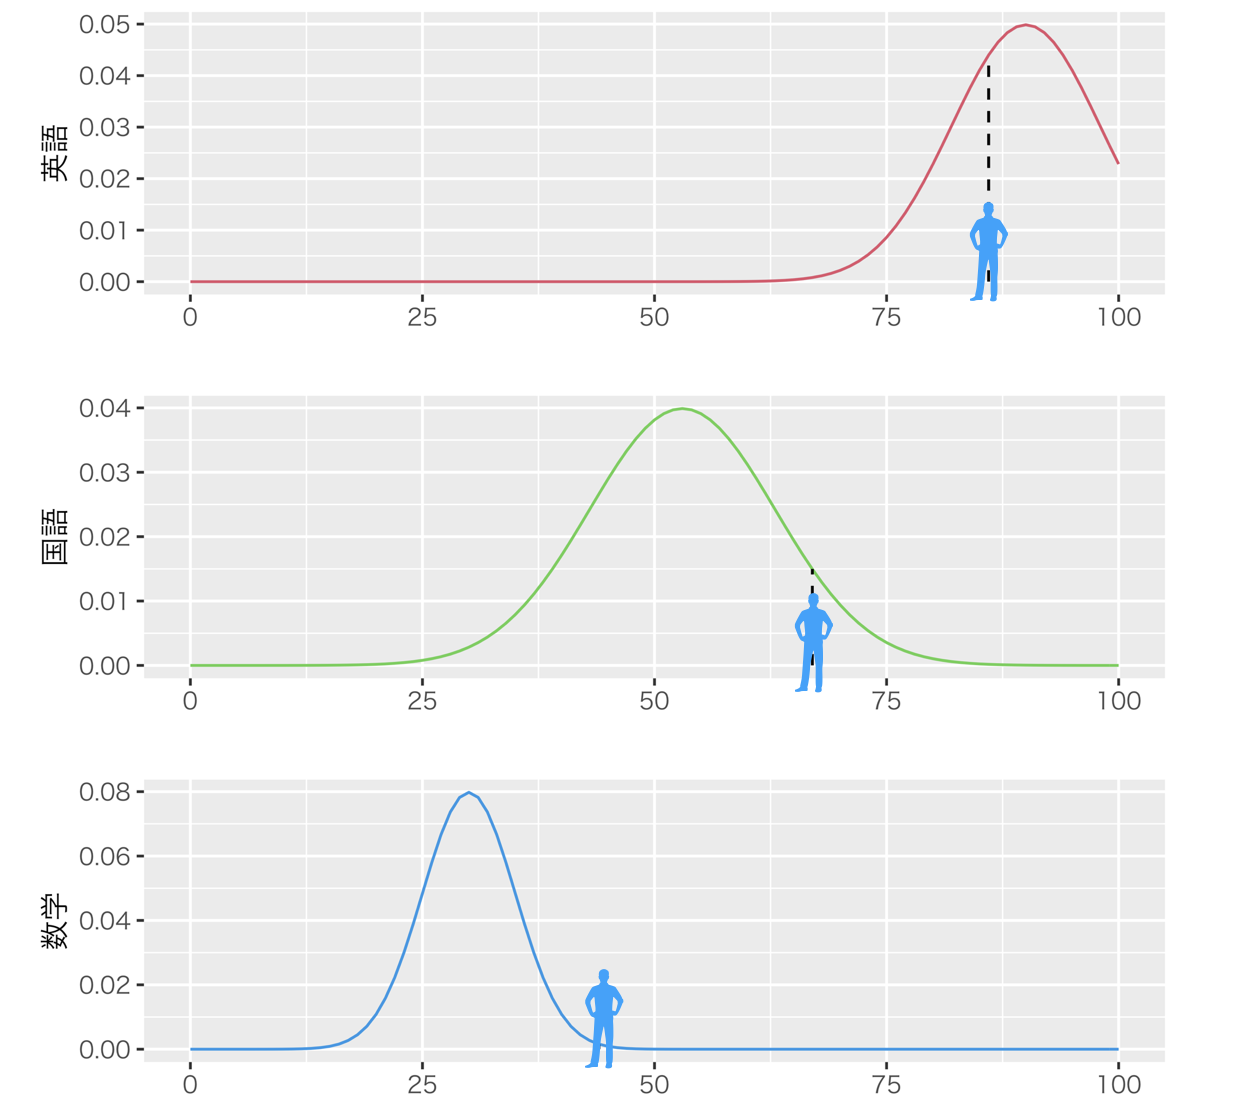
\includegraphics[keepaspectratio,width=0.8\linewidth]{../images/05_descriptives/slide04_08.png}
	\caption{Scatter and relative position of data}
	\label{fig::04_08}
\end{figure}

At the top row of Figure \ref{fig::04_08}, you can see the English distribution and the position of this person. The peak of the distribution, where the most people scored, is around 90 points, and this person is to the left of it, indicating a relatively lower score. On the second and third row, there are Japanese and mathematics scores respectively, and it can be seen that this person is relatively better at those subjects. At the same time, it is noticeable that the Japanese scores have a wider distribution, while mathematics scores have a lower average and smaller range of scatter. As Japanese scores have a wider distribution, it appears that there are people who scored higher than this person. On the other hand, since the range of mathematics scores is narrow, there are hardly any people who can score higher than this person. This implies that this person has a fairly high level of mathematical ability.
In considering relative positions, we must take into account how wide the data is spread. Therefore, we divide the deviation from the mean by the standard deviation and consider how many standard deviations away from the mean the data is. Let us call this score $z_i$, and compute it as follows.

\[ z_i = \frac{(x_i - \bar{x})}{s_x}\]

This score, $z_i$, is called a \keytermE{standardized score}, or sometimes simply a z-score. By looking at this person's grades standardized in this way, we can see that their English score is $-0.5$, their Japanese score is $+1.4$, and their math score is $+2.8$. These numbers show that the person's math proficiency stands out more than their Japanese proficiency, even though they are still proficient in both subjects.

This standardized score has an average of 0 and a variance of 1 (with a standard deviation of 1 as well). This is natural as we expressed it as the number of standard deviations from the mean. In other words, by removing the mean and standard deviation, we can compare multiple variables irrespective of their unit of measurement. For example, we previously compared scores in Japanese and math. Without standardizing the scores, the comparison would have been influenced by their scale. However, once standardized, we could compare scores even if the maximum score for Japanese was 200 and for math was 1000. This is because we are only concerned with their relative position. In the same way, we can compare variables with completely different units, such as height and weight. Even in the case of psychological data with unclear units, we can understand the relative brightness and seriousness of a person using the standardized score, and it becomes possible to compare them. Standardized scores are essential in psychological research.

You are probably familiar with "deviation score" (偏差値, hensachi) which is related to academic performance. In fact, deviation score is equivalent to z-score. However, z-score can become negative and has a smaller unit, so it is converted to have a mean of 50 and a standard deviation of 10.
\[ \text{Deviation value} = 10z_i + 50 \]
The deviation value for this person is calculated using the formula mentioned. In this example, the person's deviation values are 45 for English, 64 for Japanese, and 78 for Mathematics.

\section{Standardized Differences}
\label{std_effectsize}
The characteristic of standardized scores is that they are \underline{unitless}. For example, height can be expressed in centimeters and weight in kilograms, but naturally, no one would look at data such as 170cm and 60kg and think, "Wow, 170 is bigger than 60!" It's elementary arithmetic to not compare things with different units. It should be noted that in Japan, nobody uses the pound-yard system and globally, it is standard to use the metric and CGS unit systems in scientific papers, including those in psychology. There was even a time when it was said that "The biggest achievement of Pockemon Go! was that it got Americans to use the metric system" when it was popular in the United States.

However, if we standardize these numbers and assume a height z-score of 0.3 and a weight z-score of 1.8, we can compare them. Standardizing removes the units, so we see that they are 0.3 and 1.8 standard deviations above the mean, respectively. This means that "the weight has a larger deviation from the mean" or, in other words, "the weight is heavier relative to the height, meaning the individual is overweight." We can compare the values of 0.3 and 1.8 to come to this conclusion. If the standardized scores are negative, we know that they are below the mean, which means that if the height and weight z-scores are -0.3 and +1.8, for example, we can conclude that "the height is below the mean and the weight is above the mean, and the weight has a larger deviation from the mean," or in other words, "this individual is quite overweight."

In psychology, we measure things that are invisible\footnote{As for how we do that, we'll discuss it in the next session or in the second year course on "Applied Data Analysis".}. Variables such as the degree of depression, level of self-esteem, and strength of aggression are quantified using \keytermE{psychological scales}. These scales are developed and calculated with great care, but they do not have units. It is impossible to express the degree of depression in units such as centimeters, kilograms, decibels, lux, or joules\footnote{There is a joke that suggests pain could be quantified in units of "Hanage," which is defined as the pain caused by plucking a single nose hair, but even for something as commonplace as pain, there are no units to measure it. There was a book called New Units \citep{Hanage2017} that collected various such jokes, but unfortunately, it has gone out of print.}. When scoring, we collect data from a large number of people, and represent the distribution of scale points as a kind of standardized score, which allows us to compare scores relatively. Also, by standardizing the scores, we can compare different measures, which enables us to verify hypotheses such as "the higher the degree of depression, the stronger the aggression." Standardization is an essential process in psychology.

The standardization process is also useful when comparing between groups.

For example, let's consider the average height of men and women. Suppose the survey results show that the average height for men is 170cm and for women is 165cm. The difference is 5cm. Whether this difference is considered large or small depends on the situation, but if it is shown as a fact, it is a quantity worth considering. However, when discussing such matters, we may hear voices like "But I know many short men around me" or "My sister is taller than me." These types of problems are a so-called "subject bias," where we tend to have opinions or feelings that "not all men or women are like that" when we start talking about men or women as a subject. However, both data and opinions are not wrong. The issue of whether there is a difference when viewed as a whole group, and whether there is a difference when discussed individually, are two different levels of conversations, and cannot be compared with each other.

Moreover, the difference in perception is more noticeable when the dispersion between groups is large. Figure \ref{fig::m05_08} depicts several scenarios. The top-left graph portrays a case where the difference between groups is large, and the group dispersion is small. In such a case, the difference is noticeable, and the group overlaps are minimal, so it is apparent that there is a difference. However, what happens when the same difference exists, but the group dispersion is large? The bottom-left graph represents a scenario where there is a difference between the groups, but the group dispersion is also large. In such a case, since there is a significant overlap, it is easy to feel that "there are also other differences" when someone mentions "there is a difference between the groups." On the other hand, the right column presents a scenario where the difference is small. If the difference is small, as in the top row, and the dispersion is small as well, people tend to say "there are exceptions, but there is still a difference." However, if the difference is small while the dispersion is large, as in the bottom-right graph, many exceptions may be observed, making it difficult to perceive the difference.

\begin{figure}[ht]
    \centering
    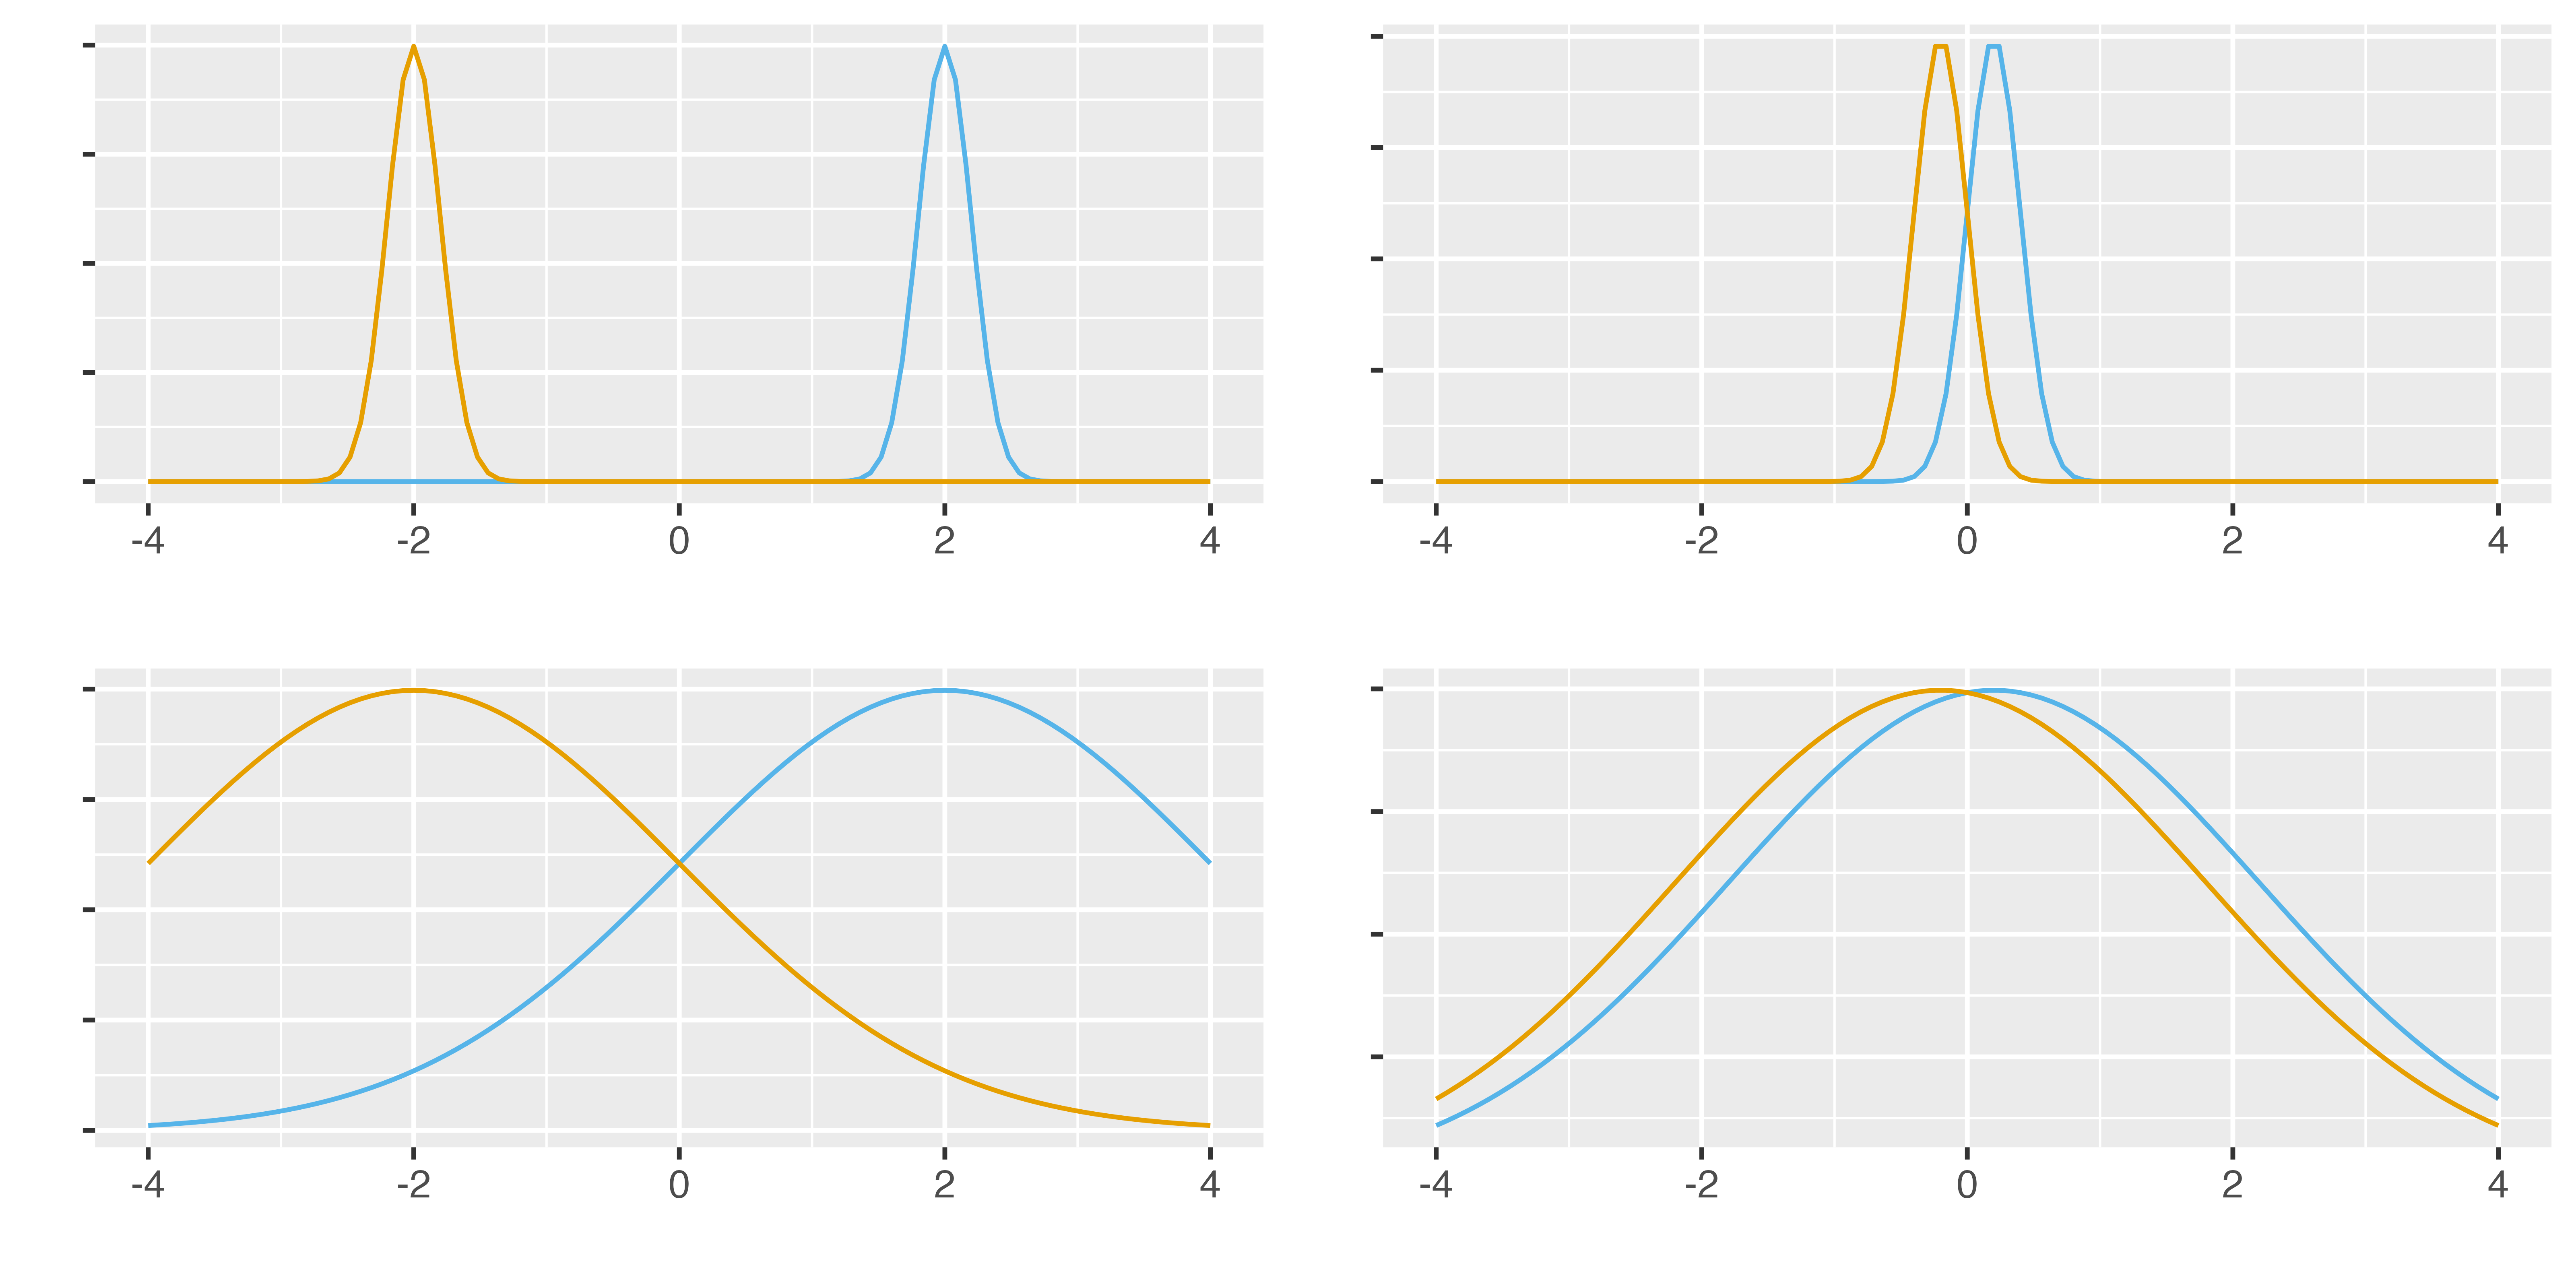
\includegraphics[keepaspectratio,width=0.8\linewidth]{../images/05_descriptives/m05_01.png}
    \caption{Pattern of differences. The left column shows larger between-group differences compared to the right column, and the lower row shows greater variance compared to the upper row.}
    \label{fig::m05_08}
\end{figure}


Talking about gender differences is a typical case of the bottom right quadrant where there is a difference when aggregated, but there is a large individual difference. If you say things like "men are strong" or "women eat less", you will immediately get flamed. While there is a difference in the average value as a fact, it often cannot express enough by itself.

What should I do then? Standardization can be helpful here again. That is, we can simply consider how much larger the difference between groups is compared to the \underline{standard deviation}. This standardized difference is particularly referred to as the \keytermE{effect size}{効果量} in Japanese.

\[ ef = \frac{\bar{X_1} - \bar{X_2}}{s_x} \]

In the example given, a value of 4 is used when the difference is large, and a value of 0.4 is used when the difference is small. The standard deviations are 2 and 0.2. When considering effect size, the upper left cell has a value of $4/0.2=20$, the lower left cell has a value of $4/2=2$, the upper right cell has a value of $0.4/0.2=2$, and the lower right cell has a value of $0.4/2=0.2$. We can see that the upper left and lower right values have very different meanings when quantified like this.

In the later stages of the course ($\to$ Lecture \ref{m17_estimation_and_test}), discussion arises on how to statistically detect differences between groups. When we say "detect differences" statistically, we are able to determine whether there are differences or not, but as seen in all cases in Figure \ref{fig::m05_08}, the difference is not zero. The important consideration is the effect size, or the difference when standardized. Of course, it is best if we can verify the substantial size when there are units present.

When doing actual data analysis, it is important to visualize and consider units and distributions, and not to rely solely on surface-level indicators.
\section{Task}
\paragraph{Calculating Representative Values} If we have data $X = \{17 , 15,  30 , 30, 43 \}$, what are the mean, median, and mode?
\paragraph{Standardization Calculation} Please fill in all the blanks in the table \ref{tbl::04_05} below.

\begin{table}[ht]
	\centering
	\caption{Bivariate $X$ and $Y$}
	\begin{tabular}{ccccccc}
		\hline
		ID                 & X   & Y  & Mean deviation of X & Mean deviation of Y & $z_x$ & $z_y$ \\
		\hline
		1                  & 149 & 37 & -2.2                & -12.4               &       &       \\
		2                  & 137 & 52 &                     &                     &       &       \\
		3                  & 164 & 67 &                     &                     &       &       \\
		4                  & 159 & 43 &                     &                     &       &       \\
		5                  & 147 & 48 &                     &                     &       &       \\
		\hline
		Mean               &     &    &                     &                     &       &       \\
		Variance           &     &    &                     &                     &       &       \\
		Standard deviation &     &    &                     &                     &       &       \\\hline
	\end{tabular}
	\label{tbl::04_05}
\end{table}




\end{document}
